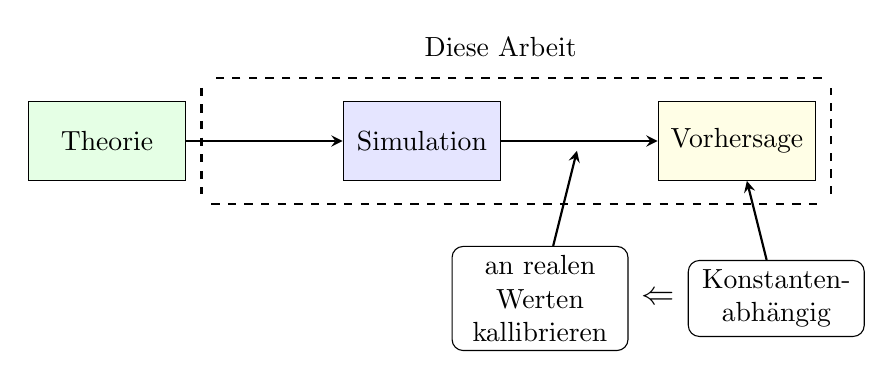
\begin{tikzpicture}
	\tikzstyle{box} = [rectangle, minimum width = 2cm, minimum height = 1cm, text centered, draw=black]
	\tikzstyle{tbox} = [rectangle, minimum width = 1cm, minimum height = 0.7cm, text centered, draw=black]
	\tikzstyle{arrow}  = [thick, ->, >=stealth]

	\node[box, fill=green!10](theorie){Theorie};

	\node[box, fill=blue!10, right of=theorie, xshift=3cm](simulation){Simulation};
	\draw[arrow] (theorie) to (simulation);

	\node[box, fill=yellow!10, right of=simulation, xshift=3cm](vorhersage){Vorhersage};
	\draw[arrow] (simulation) to (vorhersage);

	\node[tbox, rounded corners, below of=vorhersage, yshift=-1cm, xshift=0.5cm, text width=2cm](konstanten){Konstanten-\\
		abhängig};
	\draw[arrow] (konstanten) to (vorhersage);

	\node[right of=simulation, xshift=1cm](a0){};
	\node[tbox, rounded corners, below of=a0, yshift=-1cm, xshift=-0.5cm, text width=2cm](eichung){an realen Werten kallibrieren};
	\draw[arrow] (eichung) to (a0);

	\node[left of=konstanten, xshift=-0.5cm]{\large{$\Leftarrow$}};

  \node[right of=theorie, yshift=-0.8cm, xshift=0.2cm](a1){};
  \node[right of=vorhersage, yshift=-0.8cm, xshift=0.2cm](a2){};
  \node[right of=vorhersage, yshift=0.8cm, xshift=0.2cm](a3){};
  \node[right of=theorie, yshift=0.8cm, xshift=0.2cm](a4){};
  \node[above of=simulation, yshift=0.2cm, xshift=1cm](t5){Diese Arbeit};

  \draw[thick, dashed] (a1) to (a2);
  \draw[thick, dashed] (a2) to (a3);
  \draw[thick, dashed] (a3) to (a4);
  \draw[thick, dashed] (a4) to (a1);

\end{tikzpicture}
